
%%%%%%%%%%%%%% 特徴量工学の説明 %%%%%%%%%%%%
\section{特徴量工学}
図\ref{fig:EEGfootmove}と図\ref{fig:EEGhandmove}はそれぞれ足の運動想起と手の運動想起を行った際の脳波である。
いずれも0秒以前は以前はディスプレイを注視した状態であり、0秒以降に運動想起を4秒間行っている。
電極の個数は64個用いられており、全ての電極の波形が表示されている。
足の運動想起が行われているのか手の運動想起が行われているのかを脳波の生データから識別するのは困難であることが分かる。
運動想起BCIの標準的な役割は、脳波信号\(x(t)\in \mathbb R^D\)に対応した運動想起部位を識別することであるが、
そのためには脳波の生データに対して何らかの処理を施し、識別に有用な特徴を見出さねばならない。
ここに\(D\)を電極の個数である。
\begin{figure}[t]
    \centering
    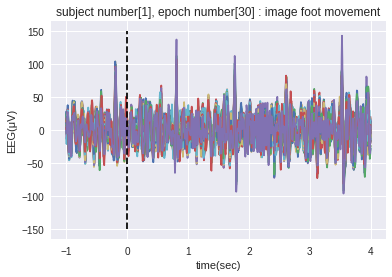
\includegraphics[width=9cm]{images/EEGfootmove.png}
    \caption{0秒〜4秒間に足の運動想起を行った際の脳波(EEG)}
    \label{fig:EEGfootmove}
\end{figure}
\begin{figure}[t]
    \centering
    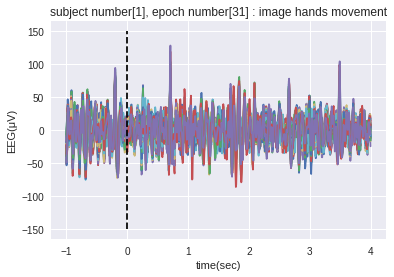
\includegraphics[width=9cm]{images/EEGhandmove.png}
    \caption{0秒〜4秒間に手の運動想起を行った際の脳波(EEG)}
    \label{fig:EEGhandmove}
\end{figure}
そこで、何らかの変換\(f(\cdot)\)を脳波信号\(x(t)\)に対して施すことで、
特徴量\(z=f(x(t))\)の獲得を目指すのが特徴量工学である。

\subsection{他分野での特徴量工学}
特徴量工学はBCIに限らず、データ解析を必要とする多くの分野で活用されている。
例えば画像処理の分野では、画像に写っている物体の輪郭を
抽出するエッジ処理や、画像に対してぼかしを入れる平滑化処理などが特徴量抽出手法として用いられる。
また音声認識の分野では、音声の周波数に重要な情報が含まれていると考え、
周波数スペクトルやケプストラムなどを特徴量として用いる試みがなされてきた。

\subsection{脳波解析における特徴量工学}
特に脳波







% \section{その他の手法}
% \subsection{スペクトログラムを特徴量とする手法}
% 運動想起型BCIでは、上記までに述べてきたCSPによる手法が非常に活発に議論されている。
% しかし、CSPによる手法は計測の際に多数の電極を用いる必要がある。
% 一方で実用上は電極が少なければ少ない程計測における負担は少なくなるため、
% 少数の電極のみを用いてBCIを構築する方法も研究がされている。
% 例として運動時、あるいは運動想起時には特定の頭皮領域に配置された電極において、
% 特定の周波数帯域にパワーの減少が生じること(事象関連脱同期)が知られているため、
% この現象に狙いを定めてBCIを構築する研究も盛んである。

% この手の手法の主な流れを示す。まず脳波信号を\(X \in \mathbb{R}^{M \times N}\)と表記する。ここに、\(M\)は電極の個数、\(N\)は計測時間点数である。
% 電極に対しての重み付け係数(空間フィルタ)$w \in \mathbb{R}^M$を何らかの方法で決定することで、
% \begin{equation*}
%     z = w^T X \in \mathbb{R}^N    
% \end{equation*}
% と変換する。次に$z$に対して短時間フーリエ変換${\cal F}(\cdot)$を行い、
% \begin{equation*}
%     A = {\cal F}(z) \in \mathbb{R}^{F\times N}
% \end{equation*}
% を獲得する。短時間フーリエ変換の代わりにウェーブレット変換などの時間周波数解析を用いる場合もある。
% スペクトログラム$A$から事象関連脱同期を見出すことができれば、ある特定の周波数帯域でのパワーを見張ることで運動の意図推定が可能となる。
% 実際、特定の周波数帯域のパワーに対して閾値を設けることで、運動意図推定を行う手法も提案されている。
% ただし、事象関連脱同期が生じる周波数帯域には個人差があることが想定されるため、スペクトログラム$A$に対して何らかの行列分解を用いて特徴量を取り出すことも提案されている。



% \subsection{Convolutional Neural Networks(ConvNets)}
% この手法に関しては\cite{deepconv}を参照されたい。